\documentclass[a4paper, 10pt]{article} 
\usepackage{natbib}
\usepackage[utf8]{inputenc}
\usepackage[portuguese,brazilian]{babel}
\usepackage[lmargin=3cm, tmargin=3cm, rmargin=2cm, bmargin=2cm]{geometry}
\usepackage[T1]{fontenc}
\usepackage{graphicx}
\usepackage{float}
\usepackage{indentfirst}
\usepackage{changepage}
\usepackage{url}
\usepackage{quoting}
\usepackage{setspace}
\setlength{\parindent}{1.5cm}

\title{Realidade Virtual - IF755}
\author{João Lucas da Silva Souza}
\date{September 2022}

\begin{document}

\maketitle

\section{Apresentação}
Uma das disciplinas eletivas da matriz curricular da graduação em Ciência de Computação pelo CIn- UFPE é a disciplina de Realidade Virtual (código IF755).  Como parte do cumprimento das competências da disciplina, os alunos desesenvolvem conhecimentos na linguagem CUDA, desenvolvida pela NVIDIA, a fim de programar para uma GPU para que consigam paralelizar o processamento do equipamento para que o equipamento tenha a melhor performance possível.

Importante frisar antes mesmo do estudo real da discplina a diferença entre Realidade Virtual e Realidade Aumentada. Enquanto a Realidade Aumentada se define por acrescentar ao mundo real elementos virtuais com o auxílio de um intermédio, como um celular, a virtual se define por um mundo completamente virtualizado que é acessado pelo usuário através de um equipamento de hardware que retira seu campo de visão do mundo exterior. De qualquer forma ao longo da escrita, ambas as definições poderão ser utilizadas como sinônimos.

\section{Realidade Virtual - sobre a disciplina}
\subsection{O que é Realidade Virtual?}
O ser humano consegue abstrair a existência da realidade através do processamento dos estímulos do mundo exterior que são entendidos pelo consciente. Contudo, é possível induzir efeitos visuais e sonoros que, mesmo não existindo materialmente em um espaço, possam receber interações diretas? A realidade virtual é incubida deste processo.

Com o auxílio da tecnologia, é possível desenvolver um ambiente completamente virtual que se sobrepõem ao espaço real do usuário. Este processo pode ser, a grosso modo, dividido por três etapas:
\begin{enumerate}
    \item Sobreposição - o que será virtualmente exibido ao usuário? A partir de determinadas interações ou requerimentos, o sistema deve decidir o que irá ser visualizado.
    \item Registro - como saber onde aumentar a realidade? A partir do pressuposto do que será exibido para o usuário, é importante limitar a definição das coordenadas da posição do objeto virtual em relação ao mundo real.
    \item Interação - como funcionará a interação com o virtual em relação ao mundo real? A partir do recebimento do estímulo virtual, o usuário tende a tomar alguma ação em relação ao objeto holográfico. Qual será a resposta dada pelo mundo virtual?
\end{enumerate}

Para Netto (2002, p. 05):

\begin{adjustwidth}{0.4\textwidth}{}
A Interface em RV envolve um controle tridimensional altamente interativo de processos computacionais. O usuário entra no espaço virtual das aplicações e visualiza, manipula e explora os dados da aplicação em tempo real, usando seus sentidos, particularmente os movimentos naturais tridimensionais do corpo. A grande vantagem é que o conhecimento intuitivo do usuário sobre o mundo físico pode ser transportado para o mundo virtual. \citep{netto2002}

\end{adjustwidth}

Concluí-se, então, que a realidade virtual é definida por tais projeções holográficas que não existem em matéria, mas são visualizadas e ouvidas pelos usuários, além de responderem à determinadas ações.
Para a construção destas características, é necessário um determinado conhecimento em construção de algorítmos e noções da geometria e da álgebra linear. Estes conceitos teóricos são de suma importância para o pleno funcionamento do sistema da realidade virtual. 
\subsection{Projeções matemáticas na Realidade Virtual}
Por se tratar de um mapeamento virtual aplicado ao mundo exterior, é necessário aplicar noções referentes à geometria na construção de um espaço virtualizado. O algoritmo deve ter a plena capacidade de entender o mundo exterior e como a aplicação de um objeto virtual pode ocorrer de uma forma que o usuário possa entender a sua visualização.

A tarefa de projetar elementos também é cabível para o funcionamento do mundo virtual. Criar um modelo simplificado do elemento que se quer projetar é necessário na construção de um algoritmo genérico, já que ele deve funcionar para qualquer ambiente externo e para qualquer elemento virtual. 

Um dispostivo de projeção arcáico, chamado de Câmera Pinhole, utiliza um dispositivo cúbico com um pequeno oríficio. A luz que entra pelo buraco na caixa consegue projetar uma imagem invertida na parede oposta ao oríficio. Resumidamente, a Câmera Pinhole é capaz de criar uma projeção do mundo exterior, uma dimensão tridimensional, em um plano bidimensional. 

\begin{figure}[h!]
    \centering
    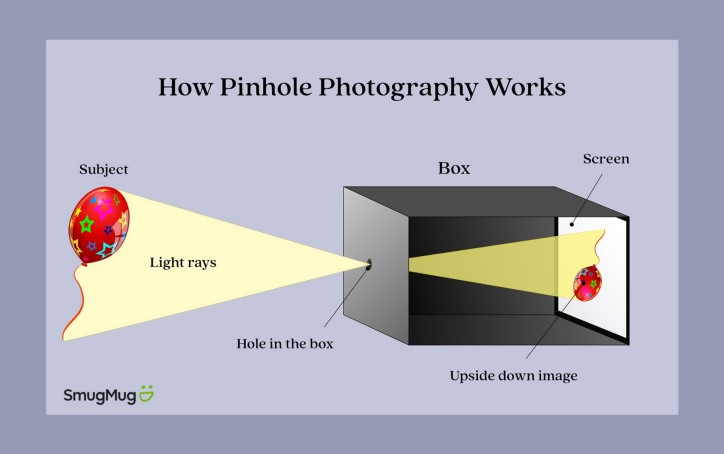
\includegraphics[width=5cm]{imagens/camera pinhole.jpg}
    \caption{Funcionamento da Câmera de Pinhole}
    \label{fig:my_label}
    \citep{campin}
\end{figure}


Assim como na câmera pinhole, o intermédio entre o mundo real e a projeção da imagem também é feito por uma câmera. Utilizando-se de dispositivos ópticos cada vez mais modernos e preparados, há a possibilidade de mapear o ambiente tridimensional e criar uma relação matemática entre o plano tridimensional (x, y, z) e o plano bidimensional (x, y). 

A grosso modo e não definindo aprofundamentos em relação aos campos da algebra e da computação gráfica, estas projeções são importantes pois são a ponte para que o algoritmo possa entender os seus planos de atuação. Serão por estes parâmetros que é possível criar um mapemento de elementos do mundo exterior e manipularmos em uma projeção virtual, ou levar uma projeção virtual para o mundo exterior através dos trabalhos da Realidade Virtual.

\subsection{Aplicações da realidade virtual ou realidade aumentada}
Para funcionalidades do nosso cotidiano, a realidade virtual pode ser uma ferramenta de auxílio que nos possibilita uma visualização virtual de algo abstrato na mente humana.

\begin{adjustwidth}{0.4\textwidth}{}
A todo  o  momento  aplicações  novas  surgem,  devido  à  demanda e capacidade  criativa  das  pessoas  através  da  RV  a  interação homem-maquina  mudou.  Devido ao avanço tecnológico de hardwares e softwa-res, a utilização de recursos de RV vem propiciando as empresas maior desempenho e menores custos. \citep{rodrigues2013}
\end{adjustwidth}

Com o auxílio de hardwares intermediários, a projeção de elementos virtuis é facilitadora no processo de trabalho. Por exemplo, é cada vez mais comum a utilização de softwares de realidade aumentada na concepção de elementos industriais ou ferramentas de trabalho.

\begin{figure}[H]
    \centering
    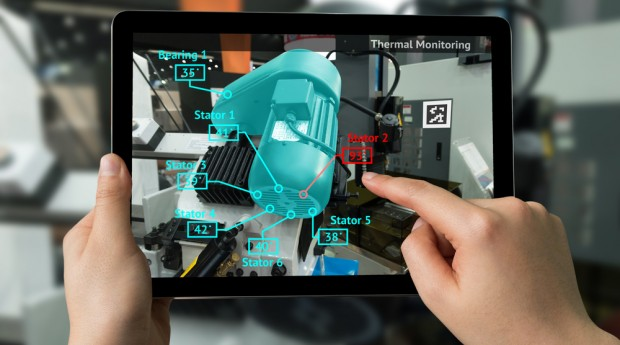
\includegraphics[width=5cm]{imagens/realidade aumentada industria.jpg}
    \caption{Realidade aumentada para a visualização de um elemento industrial}
    \label{fig:my_label}
    \citep{industry}
\end{figure}

Dispositivos com esta dinâmica são cada vez mais presentes no auxílio de projetos e ações no ambiente corporativo e industrial. Empreitadas das grandes Big Techs, como a Google com seus óculos "Google Glass" e a Microsofot com o "HoloLens", mostram que a virtualização do mundo contemporâneo é uma realidade com crescimento exponencial ano após ano. 

\begin{figure}[H]
    \centering
    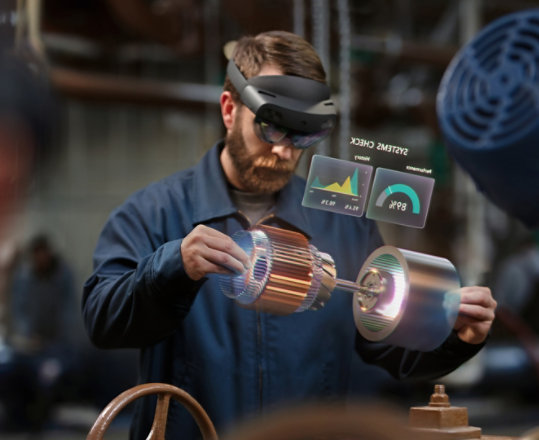
\includegraphics[width=5cm]{imagens/hololens.jpg}
    \caption{Utilização prática do "HoloLens2", óculos de realidade virtual da Microsoft}
    \label{fig:my_label}
    \citep{hololens}
\end{figure}

A realidade virtual também cria possibilidades no mapeamento de elementos do mundo exterior para o campo virtualizado. Este processo permite que o algoritmo consiga entender tais elementos e gere uma resposta ao usuário ou a um determinado dispositivo a partir do que foi visualizado.
Claro, tudo isto é feito a partir do chamado "Aprendizado de Máquina". 

É necessário ensinar ao computador o que está sendo reconhecido, o que deve ser reconhecido e como ele deve reagir aos estímulos do mundo exterior. É um processo árduo, mas abre portas para inúmeras possibilidades dentro do campo da realidade virtual.

\begin{figure}[H]
    \centering
    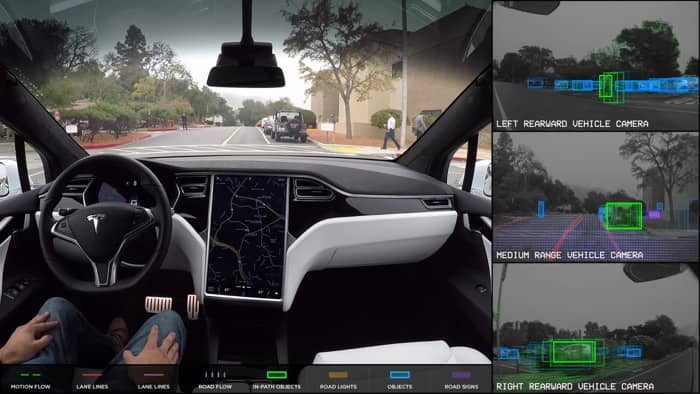
\includegraphics[width=5cm]{imagens/tesla.jpg}
    \caption{Funcionamento do "Tesla Autopilot" através do mapeamento dimensional em um carro da Tesla}
    \label{fig:my_label}
    \citep{tesla}
\end{figure}

Além de suas utilizações práticas dentro de ambientes corporativos ou em atividades rotineiras, a realidade aumentada também é uma aliada em momentos de lazer e jogos. No ano de 2016, o jogo "Pokemon GO" se tornou uma febre ao conseguir unir o mundo do jogo ao mundo real utilizando a famigerada realidade aumentada. 

Outra funcionalidade interessante é a existência de um software especializado de realidade aumentada dentro do próprio campo de pesquisa da Google. Em determinados animais, é possível encontrar a sua visualização virtual disponível para a consulta. Com esta ferramenta, um tigre pode ser virtualmente visto no dormitório de um usuário apenas com o auxílio de um celular. 

\begin{figure}[H]
    \centering
    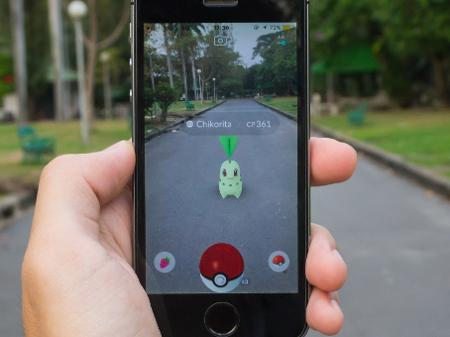
\includegraphics[width=5cm]{imagens/pokemon go.jpg}
    \caption{Realidade aumentada inserida dentro do jogo "Pokemon GO"}
    \label{fig:my_label}
    \citep{pgo}
\end{figure}
A realidade virtual é um campo amplo e que está sendo cada vez mais explorados pelas empresas e pelo grande público. O uso desta tecnologia está cada vez mais presente no cotidiano pessoal, e empreitadas como o do chamado "Metaverso" (um espaço coletivo e compartilhado completamente virtual) tendem a se tornar a nova revolução tecnológica e social das próximas décadas.

Por fim, é interessante notarmos que, para a Realidade Aumentada, não há uma imersão direta para um mundo completamente virtual, e sim os elementos abstraídos pela virtualidade são acrescidos ao mundo real \citep{liberati2018}. Utilizamos as funcionalidades de um mundo que não existe fisicamente para tornarmos as atividades do nosso cotidiano real cada vez mais práticas e dinâmicas. É a completa união entre o que é verdadeiro e o que é abstraído pelos algoritmos. 

\section{Realidade Virtual e sua relação com outras disciplinas}
Como já descrito anteriormente, os algoritmos que possibilitam a existência da Realidade Virtual são construídos a partir de conceitos vinculados à geometria e a percepção de campo. 

Este tipo de conteúdo é apresentado aos alunos logo no primeiro período durante o curso de Álgebra Linear (AVLC). Não só a percepção de Geometria Analítica, mas também noções de espaço vetorial (e seus subespaços), transformações dimensionais e sistemas lineares são fundamentais na construção de algoritmos funcionais para que o comportamento da realidade virtual tenha sentido. 

A disciplina de Processamento Gráfico também complementa os requisitos necessários para o desenvolvimento de um sistema virtual. Abordando conteúdos voltados para a visualização de elementos no campo gráfico, é fundamental que seus projetistas saibam desenvolver elementos visuais que consigam interagir com o usuário (e que também sejam de fácil entendimento e compreensão). 

Por fim, a compreensão de visão computacional dentro desta disciplina permite, por meio de intermédios, a capacidade de sistemas virtuais de interpretar o ambiente exterior e determinar uma ação a partir do que fora analisado. Como já falado anteriormente, tal capacidade dos dispositivos poderem interpretar determinados objetos é parte fundamental do aprendizado de máquina, e o Processamento Gráfico é um aliado neste tipo de algoritmo.

\newpage
\bibliographystyle{plainnat}
\bibliography{referencias}

\end{document}